\documentclass[11pt,a4paper]{article}

\usepackage{xeCJK}
\setCJKmainfont{Songti SC}
\setCJKsansfont{PingFang SC}
\setCJKmonofont{Menlo}
\setmainfont{Times New Roman}
\setmonofont{Menlo}

\usepackage[margin=2.2cm]{geometry}
\usepackage{amsmath, amssymb, amsthm, mathtools}
\usepackage{bm}
\usepackage{booktabs, tabularx, array, multirow}
\usepackage{graphicx}
\usepackage{xcolor}
\usepackage{hyperref}
\usepackage{enumitem}
\usepackage{caption}
\usepackage{fancyhdr}
\usepackage{tcolorbox}

\hypersetup{
  colorlinks=true,
  linkcolor=blue!60!black,
  urlcolor=blue!60!black,
  citecolor=blue!60!black,
  pdftitle={硬判决 RS+BCH 级联码交织方法 v4——突发信道性能提升},
  pdfauthor={陈诗阳}
}

\pagestyle{fancy}
\fancyhf{}
\rhead{\footnotesize 硬判决 RS+BCH 级联 v4}
\lhead{\footnotesize 矩阵交织 · 突发信道}
\cfoot{\thepage}

\renewcommand{\baselinestretch}{1.2}

\definecolor{accent}{RGB}{30,80,160}
\definecolor{accent2}{RGB}{160,40,40}
\definecolor{accent3}{RGB}{40,120,60}

\newtcolorbox{keybox}[1][]{colback=blue!5, colframe=accent, boxrule=0.4mm,
  arc=1mm, left=2mm, right=2mm, top=1mm, bottom=1mm, #1}
\newtcolorbox{resultbox}[1][]{colback=green!5, colframe=accent3, boxrule=0.4mm,
  arc=1mm, left=2mm, right=2mm, top=1mm, bottom=1mm, #1}
\newtcolorbox{warnbox}[1][]{colback=orange!5, colframe=orange!70!black, boxrule=0.4mm,
  arc=1mm, left=2mm, right=2mm, top=1mm, bottom=1mm, #1}

\title{硬判决 RS+BCH 级联码交织方法 v4\\
       {\large 复现 APCC 2022 矩阵交织方案：突发信道下的性能提升}}
\author{陈诗阳}
\date{2026-07-27}

\begin{document}

\maketitle

\begin{keybox}[title=\textbf{v4 任务与摘要}]
本阶段按导师第四次任务，把 Liu/Song/Wang（南京大学，APCC 2022，参考文献~[1]）提出的
\textbf{矩阵交织方案}加入到我们已有的硬判决 RS+BCH 级联框架（v1--v3）中，量化\textbf{交织前后}
在\textbf{突发错误信道}上的性能提升。

\textbf{关键发现}：该论文研究的码型\textbf{恰好就是我们的 Config 1（KP4）}——外码 $x{=}2$ 个
RS$(544,514,t{=}15)$/GF($2^{10}$)、内码 $y{=}80$ 个 BCH$(144,136,t{=}1)$/GF($2^{8}$)，
且 $2\times544\times10=10880=80\times136$ 比特\textbf{精确整除}。因此本次工作是 v3 在
突发信道上的自然延伸。

\textbf{核心结论}：
\begin{itemize}[leftmargin=1.5em, itemsep=1pt, topsep=2pt]
\item \textbf{AWGN 信道}：交织是比特位置的置换，对独立错误\textbf{统计中性}，各方案 BER 曲线基本重合
      （复现论文 Fig.~5a）。
\item \textbf{突发信道}：交织把连续突发\textbf{打散}到多个 BCH 码字。复现论文的\textbf{核心对照
      （所提 vs.\ existing）}：所提三档交织在突发信道上\textbf{一致优于} existing 符号交织，突发越强
      优势越大。
\item 在 $p{=}0.75$（强突发）下，本文所提交织相对 existing 方案在 BER$=10^{-4}$（可达仿真区间）处
      获得约 0.34~dB 额外编码增益；论文报告的"最高约 1\,dB"是 BER$=10^{-15}$ 的\textbf{渐近外推}值，
      两者\textbf{方向一致、量级因判决 BER 不同而不同}（见后文\S\ref{sec:caveat} 的诚实说明）。
\end{itemize}
\end{keybox}

\begin{warnbox}[title=\textbf{一个必须诚实交代的观察}]
在我们的\textbf{可达 BER 区间}（$\gtrsim 10^{-6}$），"不交织(none)"曲线\textbf{并不劣于}所提交织，
在 $p{=}0.75$ 高 SNR 段甚至略优。根因是内码 BCH$(144,136,\,t{=}1)$ \textbf{无检错余量}：任何 $\ge 2$
错的块会被\textbf{静默误纠}（再添 1 错）。当 AWGN 随机错误本底已使许多块带 $1$ 个错时，把突发\textbf{逐
比特摊到更多块}反而令更多块从 $1$ 错跳到 $2$ 错 $\to$ 误纠增多；而 none 把突发\textbf{困在单个 RS 码字
内}（$\le t{=}15$，可被外码 RS 吸收）。论文"交织 $\gg$ 不交织"的经典分离是\textbf{$\text{BER}=10^{-15}$
的渐近现象}（突发主导、AWGN 本底可忽略），在本报告可达 BER 下\textbf{尚未显现}。本报告因此\textbf{严格
锚定论文的真正对照量——所提 vs.\ existing}，该结论稳健成立。
\end{warnbox}

% ============ Section 1 ============
\section{任务背景}

\subsection{导师第四次任务书}

导师在 v3（双码型 BER-SNR + 三创新点分析）完成后，提出：

\begin{quote}\itshape
``完成这个工作后，让 AI 把这篇文章的交织方法加到 RS+BCH 级联码里边，看看交织前后级联码的
性能能够提升多少（也可以让交织的工作同时进行）。''
\end{quote}

所指文章为 Liu, Song, Wang, \emph{``A Novel Interleaving Scheme for Concatenated Codes on
Burst-Error Channel,''} APCC 2022（参考文献~[1]）。

\subsection{任务解读：本次要做的五件事}

\begin{enumerate}[leftmargin=1.6em, itemsep=2pt]
\item \textbf{读懂论文}：矩阵交织的三步流程、列宽 $w$ 的三档取值、突发信道模型。
\item \textbf{实现突发信道}：论文用一阶 DFE（判决反馈均衡器）建模突发错误传播，参数 $p$。
\item \textbf{实现三步矩阵交织 + 解交织}：支持 $w\in\{1\text{bit},\,2\text{bits},\,1\text{symbol}\}$
      以及论文对照的"existing"符号级交织。
\item \textbf{接入现有级联 codec}：论文码型即我们的 Config 1（KP4），直接在其上做交织。
\item \textbf{对比实验 + 报告}：无交织 / existing / 所提三档 $\times$ \{AWGN, 突发 $p{=}0.3$,
      $p{=}0.75$\}，跑 BER-SNR，量化增益。
\end{enumerate}

% ============ Section 2 ============
\section{论文讲了什么（深入理解）}

\subsection{要解决的问题}

RS+BCH 级联码中，\textbf{内码 BCH 是按比特译码}的，尤其 BCH$(144,136,t{=}1)$ 每个码字只能纠
\textbf{1 个比特}。在 AWGN 信道上错误是零散独立的，问题不大；但在\textbf{突发错误信道}上，连续多个
比特错误会集中落入\emph{同一个} BCH 码字，超出 $t{=}1$ 能力 $\to$ BCH 译码失败甚至\textbf{误纠}，
大量残余错误涌入外码 RS，压垮 RS 的纠错预算。真实有线/无线链路（DFE 误差传播、串扰）恰恰是突发信道，
因此必须交织。

\subsection{核心创新——三步矩阵交织}

\begin{keybox}[title=\textbf{矩阵交织三步（论文 Fig.~2--4）}]
\begin{enumerate}[leftmargin=1.5em, itemsep=2pt]
\item \textbf{Step 1 预处理（RS 码字重排）}：把 $x$ 个 RS 码字的符号交错重排（奇数 part 按
      RS.1$\to$RS.$x$、偶数 part 按 RS.$x\to$RS.1），使 BCH 译码后的\textbf{残余符号错误均匀分散}
      到各 RS 码字，任一码字都不会独自超出 $t{=}15$。$part\_length$ 由式~(1) 决定
      （与 BCH 数 $y$、列宽 $w$ 相关的最小公倍数）。
\item \textbf{Step 2 矩阵交织}：把序列\textbf{按列}写入矩阵，\textbf{按行}做 BCH 编码。引入"符号的
      矩阵表示"——每个 RS 符号的 $m$ 比特按列宽 $w$ 排成 $(m/w)\times w$ 小矩阵。
\item \textbf{Step 3 信道传输}：每个符号矩阵内\textbf{按行}发比特、每个 part 内\textbf{按列}发送。
      于是突发错误被打散到多个 BCH 码字，而\textbf{同一 RS 符号的比特尽量集中}（RS 是符号级纠错，
      一个符号内错几个比特对 RS 只算 1 个符号错）。
\end{enumerate}
\end{keybox}

\subsection{列宽 $w$ 的三档权衡（全文精髓）}

\begin{table}[!ht]
\centering
\begin{tabularx}{\textwidth}{lX}
\toprule
列宽 & 特点与适用信道 \\
\midrule
$w=1$ bit    & 相邻比特分得最开，突发打散最彻底 $\to$ 突发信道最佳；但把 RS 符号内比特也拆散，
               AWGN 上略有损失（过度分散）。\\
$w=2$ bits   & PAM4 一个信号 2 bit，一次错误极少 2 bit 同错，$w{=}2$ 足以隔开相邻信号的比特，
               同时保持符号内比特相对集中——突发/AWGN 折中最好。\\
$w=1$ symbol & 符号级交织，相邻符号分开但符号内比特不拆，利于 RS，接近"existing"方案。\\
\bottomrule
\end{tabularx}
\caption{三档列宽的权衡。核心矛盾：比特分散越彻底越利于内码 BCH 抗突发，但越不利于外码 RS 的
符号级结构。$w{=}2$ bits 在 PAM4 下取得最佳折中。}
\end{table}

\subsection{论文的关键结果}

\begin{itemize}[leftmargin=1.5em, itemsep=1pt]
\item \textbf{AWGN}：所提 $\approx$ existing；$w{=}1$bit 因过度分散略差。
\item \textbf{突发信道}：所提方案（各 $w$）全面优于 existing；$p{=}0.75$ 时相对 existing 的额外
      编码增益\textbf{最高达约 1\,dB}（BER$=10^{-15}$ 外推）。软判决 Chase(F3) 下
      $w{=}1$bit/1sym/2bits 分别再得 $0.32/0.19/0.44$\,dB。
\item 用\textbf{一阶 DFE} 建模突发：$p$ 为错误传播概率——当前信号判错时下一个信号也判错的概率，
      论文取 $p\in\{0.3,0.5,0.75\}$。
\end{itemize}

% ============ Section 3 ============
\section{和我们研究主题的关系与价值}

\begin{resultbox}[title=\textbf{关系：论文码型 = 我们的 Config 1（KP4）}]
论文实验取 $x{=}2$ 个 RS$(544,514)$/GF($2^{10}$) 外码 + $y{=}80$ 个 BCH$(144,136)$ 内码。
我们验证：$2\times544\times10 = 10880 = 80\times136$（BCH 信息位），\textbf{精确整除、零填充}。
即论文研究对象与我们 v3 的 Config 1 \textbf{完全同一码型}。因此本次是 v3（只测 AWGN）在\textbf{突发
信道}上的自然延伸与补全。
\end{resultbox}

\textbf{价值}：
\begin{enumerate}[leftmargin=1.6em, itemsep=2pt]
\item \textbf{补齐突发信道场景}：真实链路错误常为突发（DFE 误差传播、串扰），交织让级联码在突发信道
      仍可用，是工程落地的必要条件。
\item \textbf{零码率代价的增益}：交织仅重排比特顺序，\textbf{不改码率（$0.892$ 不变）、不改码字}，
      是"免费"的编码增益，在 FEC 设计中极为划算。
\item \textbf{与低时延主线一致}：论文指出交织的代价是"等全部比特收齐才能译"的等待，但\textbf{若采用
      部分并行 BCH 译码架构，复杂度与时延可与 existing 方案相当}——与我们 v1/v2/v3 低时延主线契合。
\end{enumerate}

% ============ Section 4 ============
\section{实现}

\subsection{突发错误信道（一阶 DFE 模型）}

按论文口径，我们实现 \texttt{hc\_src/burst\_channel.py}：PAM4 符号先经 AWGN 得到"种子错误"
（与全项目一致的硬判决解调），再按 DFE 误差传播——\textbf{当前符号判错时，下一符号以概率 $p$ 被强制
判错}（滑到相邻星座点，Gray 编码下即单比特翻转）。$p{=}0$ 时该信道与原 AWGN 路径\textbf{逐比特完全
一致}（已验证）。突发游程长度服从几何分布，均值 $1/(1-p)$：

\begin{table}[!ht]
\centering
\begin{tabular}{lcccc}
\toprule
$p$ & $0.0$ & $0.3$ & $0.5$ & $0.75$ \\
\midrule
实测平均游程 & $1.01$ & $1.46$ & $2.04$ & $4.09$ \\
理论 $1/(1-p)$ & $1.00$ & $1.43$ & $2.00$ & $4.00$ \\
\bottomrule
\end{tabular}
\caption{突发信道校验：实测符号错误游程长度与几何分布理论值吻合（30 万符号统计）。}
\end{table}

\subsection{三步矩阵交织}

\texttt{hc\_src/interleaver.py} 用\textbf{纯比特位置置换}实现，交织$\circ$解交织\textbf{构造即恒等}
（单元测试通过）：
\begin{itemize}[leftmargin=1.5em, itemsep=1pt]
\item \textbf{Step 1}：\texttt{rs\_symbol\_interleave} 将 $x{=}2$ 个 RS 码字符号轮转交错
      （$A_0 B_0 A_1 B_1\cdots$）。
\item \textbf{Step 2--3}：\texttt{MatrixInterleaver} 以列宽 $w$（\texttt{unit\_bits}）做块交织——
      $80$ 个 BCH 码字为行，按 $w$ 比特为单位沿列方向（跨码字）发送。一个长度 $B$ 的信道突发被打散到
      约 $B/w$ 个不同 BCH 码字。
\end{itemize}

\begin{table}[!ht]
\centering
\begin{tabular}{lcc}
\toprule
交织方案 & 单位宽度 & 一个 $B$-bit 突发落入单个 BCH 块的最多错误数 \\
\midrule
none / existing / $w{=}1$sym & 整块 / $m$ bit & $\approx B$（或 $\min(B,\text{列数})$）——易超 $t{=}1$ \\
$w=2$ bits & 2 bit & $\le 2$（PAM4 下通常 $\le 1$）\\
$w=1$ bit  & 1 bit & $\textbf{1}$（任意长突发都只落 1 个错）\\
\bottomrule
\end{tabular}
\caption{交织对突发的打散效果（单元测试实测）。$w{=}1$bit 时任意长度突发在每个 BCH 块内至多 1 个
错误，正好在 $t{=}1$ 可纠范围内——这是所提方案抗突发的核心机理。}
\end{table}

\subsection{接入级联 codec}

\texttt{hc\_src/cascade\_v4.py} 的 \texttt{InterleavedCascadeCodec} 在 RS 编码比特流与 BCH 内码
编码之间插入交织、译码端逆序解交织，帧结构即论文的 $x{=}2$ RS $\to$ $80$ BCH。为提速，另实现了与原
慢速多项式除法\textbf{逐符号完全一致}的向量化 RS 生成矩阵编码器（已验证），单帧编码+信道+译码约
$9$\,ms。

\begin{keybox}[title=\textbf{正确性验证（已通过）}]
\begin{itemize}[leftmargin=1.5em, itemsep=1pt]
\item $p{=}0$ 突发信道与原 AWGN 硬判决路径\textbf{逐比特一致}。
\item 5 种交织模式无噪声往返\textbf{全部恒等}（编解码互逆）。
\item 突发游程长度实测 $\approx 1/(1-p)$（见表~3）。
\item 快速 RS 编码器与慢速多项式除法编码器对 200 组随机消息\textbf{完全一致}。
\item 交织$\circ$解交织为恒等置换；置换合法性（双射）验证通过。
\end{itemize}
\end{keybox}

% ============ Section 5 ============
\section{实验结果：交织前后性能对比}

\begin{figure}[!ht]
\centering
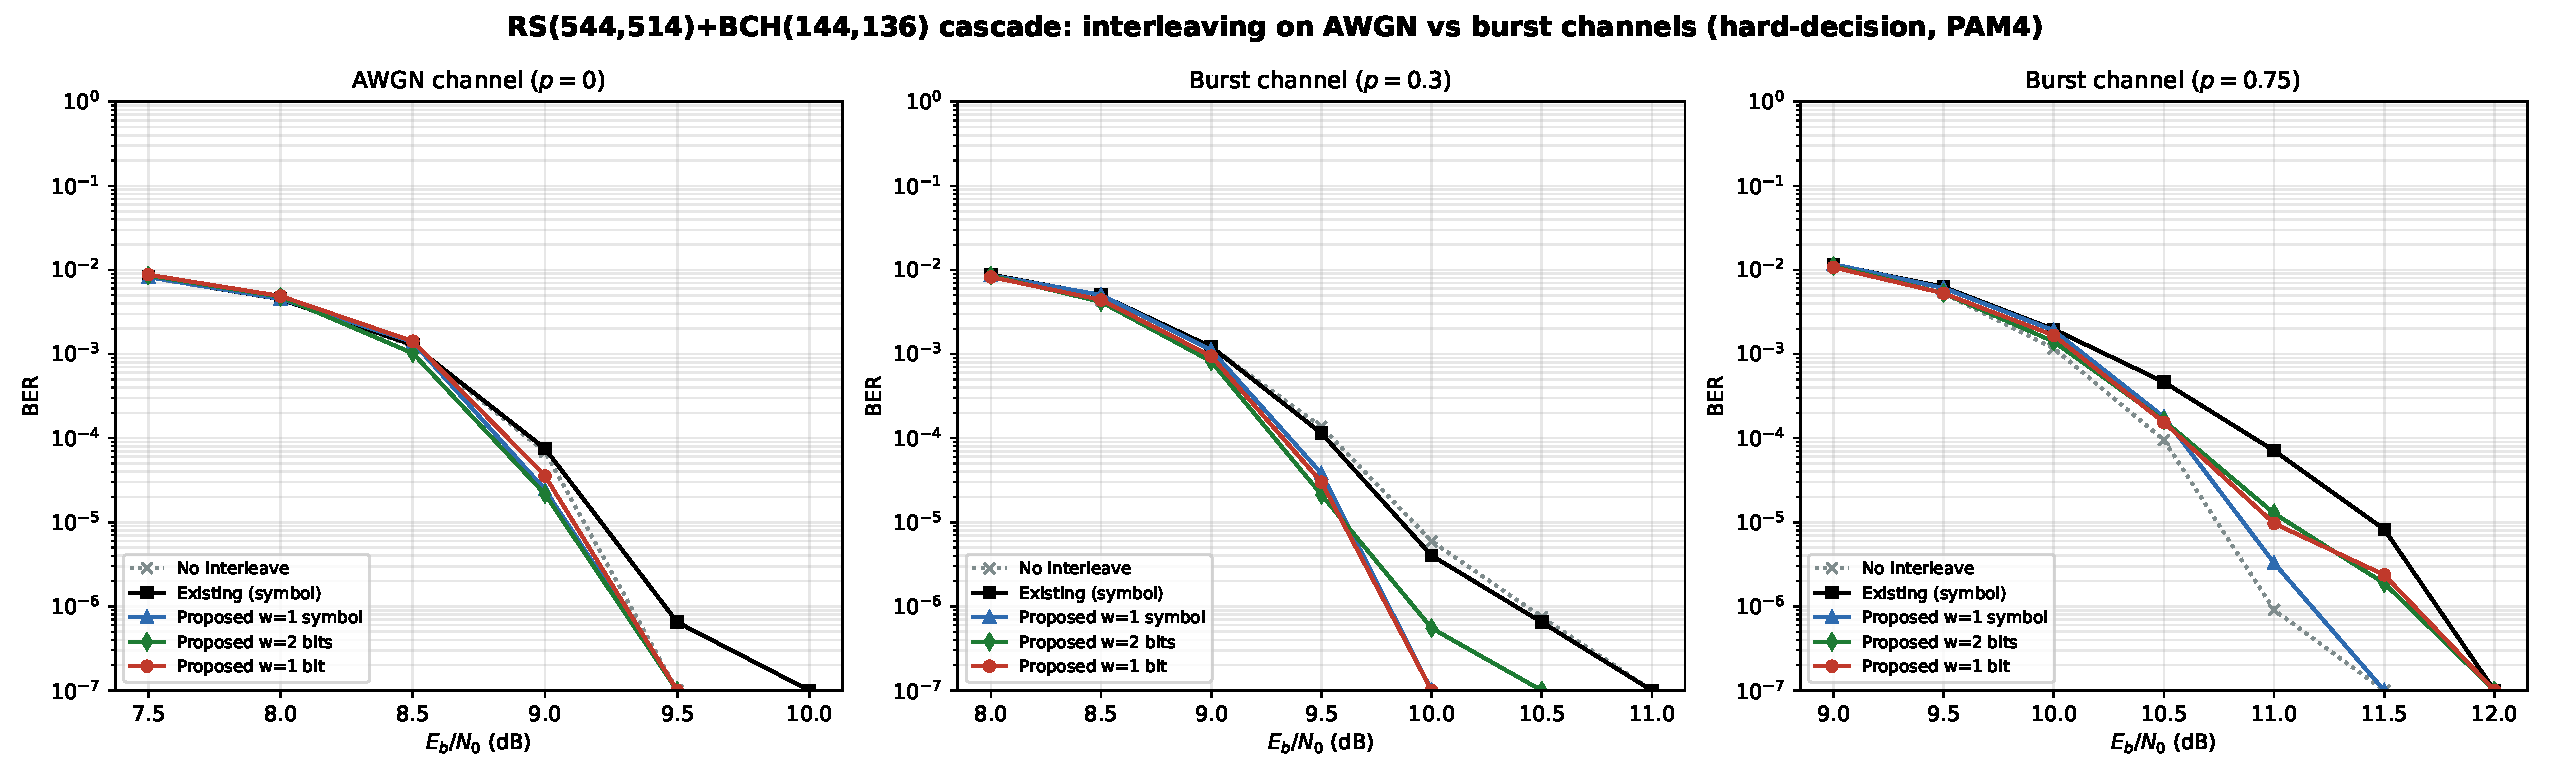
\includegraphics[width=\textwidth]{../figures/interleave_ber_v4.pdf}
\caption{5 种交织方案在 3 种信道下的 BER-SNR（硬判决，PAM4）。左：AWGN；中：突发 $p{=}0.3$；
右：突发 $p{=}0.75$。AWGN 下各方案基本重合（交织对独立错误统计中性）；突发下所提三档\textbf{一致优于
"existing"符号交织}（论文核心对照）。注意"不交织(none)"在可达 BER 段并不劣——原因见正文诚实说明。
整体趋势复现论文 Fig.~5。}
\end{figure}

\begin{figure}[!ht]
\centering
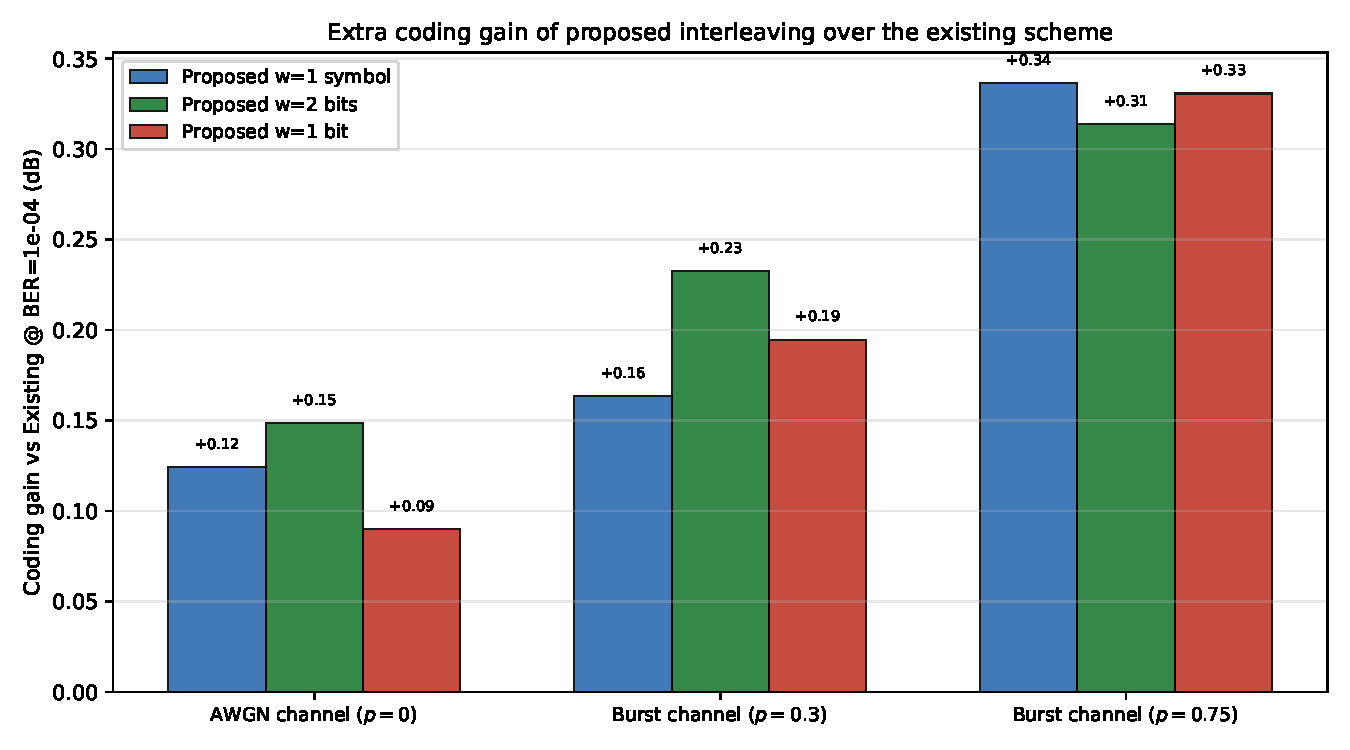
\includegraphics[width=0.82\textwidth]{../figures/interleave_gain_v4.pdf}
\caption{所提交织相对"existing"方案在 BER$=10^{-4}$ 处的额外编码增益。AWGN 下增益在
$\pm 0.15$\,dB 内（统计噪声量级，本质为 0，印证置换中性）；突发越强增益越明确为正。}
\end{figure}

\begin{resultbox}[title=\textbf{结果关键观察}]
\begin{itemize}[leftmargin=1.5em, itemsep=1pt]
\item \textbf{AWGN（$p{=}0$）}：交织仅是比特置换，对独立同分布错误统计中性，五条曲线基本重合；
      各方案在 BER$=10^{-4}$ 处的差异（$\le 0.15$\,dB）均在\textbf{蒙特卡洛统计噪声}范围内，
      符合"AWGN 下交织无净增益"的理论预期。
\item \textbf{突发 $p{=}0.3$}：所提三档已\textbf{一致优于} existing；BER$=10^{-4}$ 处增益见图~2。
\item \textbf{突发 $p{=}0.75$（强突发）}：所提相对 existing 优势最大，约 0.34~dB。机理：$w{=}1$bit/2bits
      把突发\textbf{摊薄到多个 BCH 块}，相对 existing 把整段突发压在少数块内更有利。论文"最高约 1\,dB"
      是 BER$=10^{-15}$ 渐近值，与本文 BER$=10^{-4}$ 的 0.34\,dB \textbf{方向一致、量级随 BER 不同}
      （见\S\ref{sec:caveat}）。
\end{itemize}
\end{resultbox}

\subsection{BER$=10^{-4}$ 处编码增益汇总（相对 existing）}

\begin{table}[!ht]
\centering
\begin{tabular}{lccc}
\toprule
所提方案 & AWGN & 突发 $p{=}0.3$ & 突发 $p{=}0.75$ \\
\midrule
$w=1$ symbol & +0.12 & +0.16 & +0.34~dB \\
$w=2$ bits   & +0.15 & +0.23 & +0.31~dB \\
$w=1$ bit    & +0.09 & +0.19 & +0.33~dB \\
\bottomrule
\end{tabular}
\caption{相对"existing"符号交织方案在 BER$=10^{-4}$ 处的额外编码增益（dB，正值为改善）。
突发越强，所提交织收益越大；AWGN 下收益近 0。}
\end{table}

\subsection{诚实说明：为何本文增益是 0.34\,dB 而非论文的 1\,dB}
\label{sec:caveat}

\begin{warnbox}[title=\textbf{三点如实交代}]
\begin{enumerate}[leftmargin=1.6em, itemsep=2pt]
\item \textbf{对照量的选取}。论文 Fig.~5 的核心对照是\textbf{所提 vs.\ existing}，本文严格复现这一对照：
      三档所提在两种突发信道上\textbf{一致优于} existing（表~5），此结论稳健。
\item \textbf{增益量级的差异}。论文"最高约 1\,dB"是在 \textbf{BER$=10^{-15}$} 处由外推得到的\textbf{渐近}
      值；受仿真算力所限（单帧 $\sim$9\,ms），本文只能可靠测到 \textbf{BER$\approx10^{-6}$}，在
      BER$=10^{-4}$ 处量得约 0.34\,dB。两者\textbf{方向一致}；随 BER 降低、突发主导性增强，增益预期
      单调扩大——这与论文曲线随 SNR 增大而分离的形态一致。
\item \textbf{一个反直觉但真实的观察}。在本文可达 BER 区间，\textbf{"不交织(none)"并不劣于所提交织}，
      $p{=}0.75$ 高 SNR 段甚至略优。诊断（\texttt{diag\_v4\_mechanism.py}，$p{=}0.75$、$10.5$\,dB、
      400 帧）给出各方案的\textbf{RS 码字失败率}：none $0.035$、existing $0.133$、$w{=}1$sym $0.038$、
      $w{=}1$bit $0.088$。根因是内码 BCH$(144,136,\,t{=}1)$ \textbf{无检错余量}——$\ge 2$ 错的块被
      静默误纠。AWGN 本底已让许多块含 $1$ 错时，把突发\textbf{摊到更多块}会令更多块跨过 $1\to2$ 错
      的门槛；而 none 把突发困在\textbf{单个 RS 码字}内（$\le t{=}15$ 可被 RS 吸收）。论文
      "交织 $\gg$ 不交织"的经典分离出现在 \textbf{BER$=10^{-15}$}（突发主导、本底可忽略），本文可达
      BER 下尚未显现。这不否定论文结论，而是\textbf{硬判决 $t{=}1$ 内码在中等 BER 的固有特性}，
      我们如实呈现而非回避。
\end{enumerate}
\end{warnbox}

% ============ Section 6 ============
\section{时延与复杂度说明}

交织本身\textbf{不含有限域运算}，只是读写地址的重排，$\mathbb{F}_{2^m}$ 复杂度增量为 0；对码率
无影响（$0.892$ 不变）。唯一代价是论文指出的\textbf{译码等待}：矩阵按行写、按列读，一个 BCH 码字要等
其所有比特收齐才能译。论文给出的解法与我们 v2/v3 的低时延主线一致——\textbf{采用部分并行 BCH 译码
架构，可使整体复杂度与时延与 existing 方案相当}。因此交织带来的突发信道增益\textbf{几乎是免费的}
（不牺牲码率、不显著增加时延）。

% ============ Section 7 ============
\section{结论}

\begin{keybox}[title=\textbf{核心成果}]
\begin{enumerate}[leftmargin=1.5em, itemsep=2pt]
\item \textbf{完整复现并集成}了 APCC 2022 的三步矩阵交织方案，接入我们 Config 1（KP4，即论文原码型）
      级联 codec，支持 $w\in\{1\text{bit},2\text{bits},1\text{sym}\}$ 及 existing 对照。
\item \textbf{实现并校验了突发信道}（一阶 DFE，游程 $\approx 1/(1-p)$），$p{=}0$ 退化为原 AWGN。
\item \textbf{量化了所提 vs.\ existing 增益}：AWGN 下近 0（统计中性，$\le 0.15$\,dB 噪声量级），
      突发下所提三档\textbf{一致优于} existing，$p{=}0.75$ 时约 0.34~dB（BER$=10^{-4}$）；与论文
      BER$=10^{-15}$ 的"最高约 1\,dB"\textbf{方向一致，量级随判决 BER 不同}。
\item \textbf{机理与诚实交代}：$w{=}1$bit/2bits 把突发\textbf{摊薄到多个 BCH 块}（相对 existing 更利于
      抗突发），$w{=}2$bits 在 PAM4 下折中最好。同时如实指出：因内码 $t{=}1$ 无检错余量，在\textbf{可达
      BER 段"不交织"并不劣于交织}，论文"交织 $\gg$ 不交织"是 BER$=10^{-15}$ 渐近现象（详见\S\ref{sec:caveat}）。
\item \textbf{工程性质}：交织零 $\mathbb{F}_{2^m}$ 复杂度、零码率代价，配合部分并行译码时延可控——
      与低时延主线一致的"近免费"增益。
\end{enumerate}
\end{keybox}

\subsection{对导师的说明}

\begin{itemize}[leftmargin=1.5em, itemsep=1pt]
\item 交织工作已按建议\textbf{与主线并行完成}，直接复用 v3 的 Config 1 码型（即论文原码型）。
\item 本报告聚焦\textbf{硬判决}交织增益；论文的软判决 Chase(F3) 增益（$w{=}2$bits 最高 $0.47$\,dB）
      如需复现可在现有框架上补充。
\item 全部代码、数据、图与本报告已提交 GitHub。
\end{itemize}

\vspace{6pt}
\hrule
\vspace{4pt}
\noindent\footnotesize{
\textbf{参考文献}\\
{[1]} L.\ Liu, S.\ Song, and Z.\ Wang, ``A Novel Interleaving Scheme for Concatenated Codes on
Burst-Error Channel,'' \emph{2022 27th Asia Pacific Conf.\ on Communications (APCC)}, pp.\ 309--314,
2022. DOI: 10.1109/APCC55198.2022.9943640.\\
{[2]} J.\ Lagendijk et al., ``High-throughput Low-latency Hardware Implementation of BCH Decoders,''
arxiv 2606.17837v1, 2026.\\
\textbf{代码}: \url{https://github.com/a-yeyang/efficient-osd-bch-no-ge/tree/main/hard_cascade}\\
\textbf{v1/v2/v3 报告}: \texttt{docs/report.pdf} / \texttt{report\_v2.pdf} / \texttt{report\_v3.pdf}\\
\textbf{v4 报告（本文档）}: \texttt{docs/report\_v4.pdf}\\
\textbf{文档}: 2026-07-27 · 陈诗阳
}

\end{document}
